\documentclass[tikz,border=10pt]{standalone}
\usepackage{tikz}
\usetikzlibrary{positioning}
\usepackage{tikz-feynman}
\begin{document}

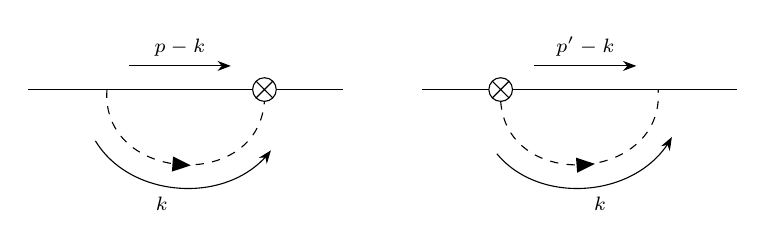
\begin{tikzpicture}
	\begin{feynman}
		%% fig d
		\vertex (d1) at (0,0);
		\vertex[right =1cm  of d1] (d2);
		\vertex[right =2cm  of d1] (d3);
		\vertex[right =3cm  of d1, crossed dot,anchor=center] (d4){};
		\vertex[right =4cm  of d1] (d5);
		\node[above =0.5 cm  of d5] {};
		%% fig e
		\vertex[above right =0 cm and 5 cm of d1] (e1);
		\vertex[right =1cm  of e1, crossed dot,anchor=center] (e2){};
		\vertex[right =2cm  of e1] (e3);
		\vertex[right =3cm  of e1] (e4);
		\vertex[right =4cm  of e1] (e5);
		\node[above =0.5cm of e5] {};
		% 对各个顶点连线
		\diagram*{
		{
		[edge=plain]
		(d1) --  (d2)--[momentum = {\scriptsize \(p-k\)}](d4)-- (d5),
		(e1) --  (e2)--[momentum = {\scriptsize \(p^{\prime}-k\)}] (e4)-- (e5),
		},
		% 介子连线
		{
		[edge= charged scalar]
		(d2) --[half right,momentum' ={\scriptsize \(k\)}](d4),
		(e2) --[half right,momentum' ={\scriptsize \(k\)}](e4),
		}
		};
	\end{feynman}
\end{tikzpicture}

\end{document}

